\documentclass[10pt,journal,compsoc,onecolumn]{IEEEtran}
\usepackage[utf8]{inputenc}
\usepackage{amsmath,amsfonts,amssymb}
\usepackage{amsthm}
\usepackage{graphicx}
\usepackage{cite}
\usepackage{textcomp}
\usepackage{tikz}
\usetikzlibrary{arrows,positioning,shapes.geometric}
\usepackage{booktabs}
\usepackage{url}

\newtheorem{theorem}{Theorem}
\newtheorem{lemma}[theorem]{Lemma}
\newtheorem{definition}[theorem]{Definition}
\newtheorem{corollary}[theorem]{Corollary}

\begin{document}

\title{The Backtracking Paradigm: Mathematical Formalization, Complexity Analysis, and Systems Stack Dynamics in Combinatorial Search}

\IEEEtitleabstractindextext{%
\begin{abstract}
This paper presents a formal mathematical and systems-level analysis of backtracking algorithms. We investigate three canonical combinatorial problems: (1) Generating Valid Parentheses, modeled as Dyck paths and bounded by Catalan numbers, whose asymptotic limits we derive via Stirling's approximation; (2) Subset Generation (Power Set construction), modeled as binary decision tree exploration; and (3) Permutation Generation, analyzed through factorial growth and resolved via visited-state and swap-based backtracking models. For each problem, we present rigorous proofs of correctness, asymptotic complexity bounds, and production-ready Java implementations. Finally, we dissect the low-level systems dynamics of backtracking, tracing stack-frame activation records and illustrating the mechanical necessity of state restoration in shared memory architectures.
\end{abstract}

\begin{IEEEkeywords}
binary trees, algorithms, data structures, computational complexity, tree traversal, recursive algorithms, formal analysis
\end{IEEEkeywords}
}

\maketitle
\IEEEdisplaynontitleabstractindextext
\IEEEpeerreviewmaketitle

\section{Introduction}
\label{sec:intro}

Combinatorial search problems are prevalent across theoretical computer science, operations research, and automated theorem proving. Often, these problems exhibit a search space that grows exponentially, $\mathcal{O}(2^N)$, or factorially, $\mathcal{O}(N!)$, with respect to the input size $N$. While brute-force search is guaranteed to find a solution by visiting every candidate configuration, it becomes computationally intractable for even modest values of $N$. 

The backtracking paradigm is a highly refined systematic search technique that optimizes combinatorial exploration. Instead of generating complete candidate configurations and evaluating them post-hoc, backtracking constructs candidates incrementally. It models the search space as a tree and traverses it using Depth-First Search (DFS). At each step, a bounding function (or predicate) evaluates the partial candidate. If the predicate determines that the current partial configuration cannot be extended to a valid solution, the algorithm prunes the entire subtree, avoiding the exploration of invalid paths. The algorithm then reverts the latest state change (the "backtracking step") and attempts the next choice.

Formally, let a solution be represented as a vector $\mathbf{X} = (x_1, x_2, \ldots, x_k)$, where each coordinate $x_i$ is chosen from a finite domain $S_i$. Let $P(x_1, \ldots, x_i)$ be a predicate mapping to $\{\text{true}, \text{false}\}$, representing the feasibility of the prefix. If $P(x_1, \ldots, x_i) = \text{false}$, the search branches from node $(x_1, \ldots, x_i)$ are pruned.

This paper presents an exhaustive formalization of three fundamental backtracking problems:
\begin{enumerate}
    \item \textbf{Generating Valid Parentheses (\S\ref{sec:parentheses}):} Modeling valid parentheses as Dyck paths, bounding the search space using Catalan numbers, proving the asymptotic limits via Stirling's approximation, and implementing a pruned DFS.
    \item \textbf{Power Set Generation (\S\ref{sec:subsets}):} Formalizing subset generation as a binary decision tree of size $2^N$ and analyzing backtracking state management.
    \item \textbf{Permutation Generation (\S\ref{sec:permutations}):} Analyzing factorial growth and implementing visited-array and swap-based backtracking paradigms for workout scheduling customization.
    \item \textbf{Systems Stack Invariants (\S\ref{sec:systems}):} A low-level execution trace illustrating stack-frame activation records and the mechanical necessity of state restoration.
\end{enumerate}

%% ============================================================
\section{Generating Valid Parentheses: Dyck Paths and Catalan Bounds}
\label{sec:parentheses}

The problem of generating all combinations of well-formed parentheses of length $2N$ given $N$ pairs of parentheses is isomorphic to enumerating monotonic lattice paths in a grid that do not cross the diagonal.

\subsection{Mathematical Model and Dyck Invariants}
Let $S = s_1 s_2 \ldots s_{2N}$ be a string of length $2N$ over the alphabet $\Sigma = \{\text{'('}, \text{')'}\}$. Define a valuation mapping $v: \Sigma \to \{1, -1\}$ as:
\begin{equation}
v(s_j) = \begin{cases} 
1 & \text{if } s_j = \text{'('} \\
-1 & \text{if } s_j = \text{')'} 
\end{cases}
\end{equation}
A string $S$ represents a well-formed parenthesis combination if and only if it satisfies two conditions:
\begin{align}
\sum_{j=1}^{2N} v(s_j) &= 0 \label{eq:dyck1} \\
\forall i \in \{1, \ldots, 2N\}, \quad \sum_{j=1}^{i} v(s_j) &\ge 0 \label{eq:dyck2}
\end{align}
Equation~\eqref{eq:dyck1} guarantees that the number of open and closed parentheses is equal. Equation~\eqref{eq:dyck2} ensures that at no prefix does the number of closed parentheses exceed the number of open parentheses. A string satisfying these rules is a \emph{Dyck word}, and the corresponding path in $\mathbb{Z}^2$ is a \emph{Dyck path}.

The total number of valid Dyck paths of length $2N$ is given by the $N$-th Catalan number $C_N$:
\begin{equation}
C_N = \frac{1}{N+1}\binom{2N}{N} = \frac{(2N)!}{(N+1)!N!}
\end{equation}

\subsection{Asymptotic Complexity via Stirling's Approximation}
To appreciate the search space reduction achieved by backtracking compared to a naive brute-force generation of all $2^{2N}$ strings, we compute the asymptotic behavior of $C_N$. Stirling's approximation states that:
\begin{equation}
n! \approx \sqrt{2\pi n} \left(\frac{n}{e}\right)^n
\end{equation}
Applying this to the terms in the Catalan formula:
\begin{align}
C_N &= \frac{(2N)!}{(N+1)N!N!} \approx \frac{(2N)!}{N \cdot (N!)^2} \\
&\approx \frac{\sqrt{4\pi N} \left(\frac{2N}{e}\right)^{2N}}{N \left( \sqrt{2\pi N} \left(\frac{N}{e}\right)^N \right)^2} = \frac{2\sqrt{\pi N} \left(\frac{2N}{e}\right)^{2N}}{N \cdot 2\pi N \left(\frac{N}{e}\right)^{2N}} \\
&= \frac{2\sqrt{\pi N} \cdot 4^N \cdot \left(\frac{N}{e}\right)^{2N}}{2\pi N^2 \left(\frac{N}{e}\right)^{2N}} = \frac{4^N}{N^{3/2}\sqrt{\pi}}
\end{align}
Thus, the cardinality of the search space grows at:
\begin{equation}
C_N \sim \frac{4^N}{N^{3/2}\sqrt{\pi}}
\end{equation}
This is significantly smaller than the brute-force binary string search space of $4^N$.

\subsection{Algorithm Design and Bounding Predicate}
The backtracking algorithm maintains three state variables: the current accumulated string $S$, the count of open parentheses used $o$, and the count of closed parentheses used $c$. Starting from $S = \epsilon$ and $o = c = 0$, we branch recursively by appending either '(' or ')'.
The bounding predicates that prune invalid branches are:
\begin{enumerate}
    \item \textbf{Open Limit:} We cannot append '(' if $o \ge N$.
    \item \textbf{Well-Formed Balance:} We cannot append ')' if $c \ge o$. This enforces Equation~\eqref{eq:dyck2} in real-time.
\end{enumerate}

\subsection{Java Reference Implementation}
\begin{verbatim}
import java.util.ArrayList;
import java.util.List;

public class ParenthesisGenerator {
    public List<String> generateParenthesis(int N) {
        List<String> result = new ArrayList<>();
        backtrack(result, new StringBuilder(), 0, 0, N);
        return result;
    }

    private void backtrack(List<String> result, StringBuilder current, 
                           int open, int close, int max) {
        if (current.length() == max * 2) {
            result.add(current.toString());
            return;
        }

        if (open < max) {
            current.append('(');
            backtrack(result, current, open + 1, close, max);
            current.deleteCharAt(current.length() - 1); // Backtracking step
        }
        if (close < open) {
            current.append(')');
            backtrack(result, current, open, close + 1, max);
            current.deleteCharAt(current.length() - 1); // Backtracking step
        }
    }
}
\end{verbatim}

\subsection{Complexity Analysis}
\begin{itemize}
    \item \textbf{Time Complexity:} The recursion tree has $C_N$ leaf nodes, and the path from the root to each leaf is of length $2N$. The intermediate nodes in the recursion tree also scale proportionally to the number of leaves. Thus, the total time complexity is:
    \begin{equation}
    T(N) = \mathcal{O}(N \cdot C_N) = \mathcal{O}\left( \frac{4^N}{N^{1/2}} \right)
    \end{equation}
    \item \textbf{Space Complexity:} The maximum recursion depth is $2N$, corresponding to the height of the state space tree. The call stack holds $2N$ stack frames, and the \texttt{StringBuilder} holds at most $2N$ characters. Excluding the output memory, the auxiliary space complexity is:
    \begin{equation}
    S_{\text{aux}}(N) = \mathcal{O}(N)
    \end{equation}
\end{itemize}

%% ============================================================
\section{Power Set Construction: Subset Generation}
\label{sec:subsets}

Given a set of $N$ distinct elements, generating all subsets (the Power Set) is a canonical combinatorial problem characterized by a complete binary search tree.

\subsection{Mathematical Model of the Power Set}
Let $S = \{a_1, a_2, \ldots, a_N\}$ be a set of size $N$. The Power Set $\mathcal{P}(S)$ is the set of all subsets of $S$. The cardinality of $\mathcal{P}(S)$ is:
\begin{equation}
|\mathcal{P}(S)| = 2^N
\end{equation}
We can represent any subset $A \subseteq S$ as a binary vector $\mathbf{v} = (v_1, v_2, \ldots, v_N) \in \{0, 1\}^N$, where:
\begin{equation}
v_i = \begin{cases}
1 & \text{if } a_i \in A \\
0 & \text{if } a_i \notin A
\end{cases}
\end{equation}
The mapping between $\{0, 1\}^N$ and $\mathcal{P}(S)$ is bijective. The search space is a complete binary tree of height $N$, containing $2^{N+1}-1$ nodes.

\subsection{Algorithm Design and State Propagation}
The backtracking algorithm walks through the array element-by-element using an index variable \texttt{index}. At each step, it branches into two decisions:
\begin{enumerate}
    \item \textbf{Include:} Append $a_{\text{index}}$ to the active list, recurse on \texttt{index + 1}, and then pop $a_{\text{index}}$ to clean the state.
    \item \textbf{Exclude:} Recurse on \texttt{index + 1} without modifying the active list.
\end{enumerate}

\subsection{Java Reference Implementation}
\begin{verbatim}
import java.util.ArrayList;
import java.util.List;

public class SubsetGenerator {
    public List<List<Integer>> subsets(int[] nums) {
        List<List<Integer>> result = new ArrayList<>();
        backtrack(result, new ArrayList<>(), nums, 0);
        return result;
    }

    private void backtrack(List<List<Integer>> result, List<Integer> current, 
                           int[] nums, int index) {
        if (index == nums.length) {
            result.add(new ArrayList<>(current)); // Deep copy subset
            return;
        }

        // Branch 1: Include nums[index]
        current.add(nums[index]);
        backtrack(result, current, nums, index + 1);
        current.remove(current.size() - 1); // Backtracking step (state restoration)

        // Branch 2: Exclude nums[index]
        backtrack(result, current, nums, index + 1);
    }
}
\end{verbatim}

\subsection{Complexity Analysis}
\begin{itemize}
    \item \textbf{Time Complexity:} There are $2^N$ subsets. At each leaf node, we copy the current list to the output, which takes $\mathcal{O}(K)$ time, where $K$ is the size of the subset. The average size of a subset is:
    \begin{equation}
    E[K] = \frac{1}{2^N}\sum_{k=0}^{N} k \binom{N}{k} = \frac{N}{2}
    \end{equation}
    Therefore, the total time complexity is:
    \begin{equation}
    T(N) = \mathcal{O}(N \cdot 2^N)
    \end{equation}
    \item \textbf{Space Complexity:} The height of the recursion tree is $N$. The active list \texttt{current} uses at most $O(N)$ space. Excluding the output list, the auxiliary space complexity is:
    \begin{equation}
    S_{\text{aux}}(N) = \mathcal{O}(N)
    \end{equation}
\end{itemize}

%% ============================================================
\section{Permutation Generation: Visited-State and Swap-Based Models}
\label{sec:permutations}

Generating all permutations of a sequence is a fundamental problem where the search space grows factorially. We explore this problem within the context of a fitness application (FitBit) that seeks to randomize exercise sequences.

\subsection{Mathematical Model of Permutations}
Let $A = [a_1, a_2, \ldots, a_N]$ be a sequence of $N$ distinct elements. A permutation of $A$ is a bijective function $\sigma: \{1, \ldots, N\} \to \{1, \ldots, N\}$. The total number of permutations is:
\begin{equation}
N! = \prod_{i=1}^{N} i
\end{equation}
By Stirling's approximation, the search space grows at:
\begin{equation}
N! \sim \sqrt{2\pi N} \left( \frac{N}{e} \right)^N
\end{equation}
This super-exponential growth requires efficient state manipulation algorithms to prevent memory leaks and unnecessary copies during search.

\subsection{Algorithm 1: Visited-Set Method}
The first approach keeps track of a global boolean array \texttt{visited} of size $N$. At each step, we iterate from $0$ to $N-1$. If the element at index $i$ has not been visited, we mark it as visited, append it to our active permutation path, recurse, and then revert the visited status and pop the element.

\subsubsection{Java Reference Implementation}
\begin{verbatim}
import java.util.ArrayList;
import java.util.List;

public class PermutationVisited {
    public List<List<Integer>> permute(int[] nums) {
        List<List<Integer>> result = new ArrayList<>();
        boolean[] visited = new boolean[nums.length];
        backtrack(result, new ArrayList<>(), nums, visited);
        return result;
    }

    private void backtrack(List<List<Integer>> result, List<Integer> current, 
                           int[] nums, boolean[] visited) {
        if (current.size() == nums.length) {
            result.add(new ArrayList<>(current));
            return;
        }

        for (int i = 0; i < nums.length; i++) {
            if (visited[i]) continue;

            current.add(nums[i]);
            visited[i] = true;
            backtrack(result, current, nums, visited);
            
            // Backtracking step
            visited[i] = false;
            current.remove(current.size() - 1);
        }
    }
}
\end{verbatim}

\subsection{Algorithm 2: In-Place Swap Method}
The second approach avoids the auxiliary \texttt{visited} array by swapping elements directly in the input array. At recursion depth \texttt{start}, we swap the element at index \texttt{start} with every element at index $i$ (where $i \ge \text{start}$), recurse on $\text{start}+1$, and then swap them back to restore the original array order.

\subsubsection{Java Reference Implementation}
\begin{verbatim}
import java.util.ArrayList;
import java.util.List;

public class PermutationSwap {
    public List<List<Integer>> permute(int[] nums) {
        List<List<Integer>> result = new ArrayList<>();
        List<Integer> list = new ArrayList<>();
        for (int n : nums) list.add(n);
        backtrack(result, list, 0);
        return result;
    }

    private void backtrack(List<List<Integer>> result, List<Integer> nums, int start) {
        if (start == nums.size()) {
            result.add(new ArrayList<>(nums));
            return;
        }

        for (int i = start; i < nums.size(); i++) {
            java.util.Collections.swap(nums, start, i);
            backtrack(result, nums, start + 1);
            java.util.Collections.swap(nums, start, i); // Backtracking step
        }
    }
}
\end{verbatim}

\subsection{Complexity Analysis}
\begin{itemize}
    \item \textbf{Time Complexity:} The total number of leaf nodes in the recursion tree is exactly $N!$. The height of the tree is $N$. Copying a permutation of size $N$ at each leaf node takes $\mathcal{O}(N)$ time. The total time complexity is:
    \begin{equation}
    T(N) = \mathcal{O}(N \cdot N!)
    \end{equation}
    \item \textbf{Space Complexity:} The maximum stack depth is $N$. For the swap-based method, no extra array is allocated. Thus, the auxiliary space complexity (excluding output storage) is:
    \begin{equation}
    S_{\text{aux}}(N) = \mathcal{O}(N)
    \end{equation}
\end{itemize}

%% ============================================================
\section{Systems Perspective: Stack Frame Dynamics and State Cleanup}
\label{sec:systems}

Understanding backtracking requires analyzing how recursive functions interact with the program runtime stack.

\subsection{Activation Records (Stack Frames)}
When a function is called, the CPU allocates a block of memory on the stack known as an \emph{activation record} or \emph{stack frame}. A standard stack frame contains:
\begin{itemize}
    \item \textbf{Local Variables:} Local identifiers (e.g., loop counter $i$ inside the permutation generator).
    \item \textbf{Parameters:} Value copies or reference addresses passed to the function (e.g., the reference to the \texttt{current} list).
    \item \textbf{Frame Pointer (EBP/RBP):} A pointer to the caller's stack frame.
    \item \textbf{Return Address:} The address of the next machine instruction to execute in the caller function after the callee returns.
\end{itemize}

\subsection{The Execution Trace of State Pollution}
Consider what happens during the execution of \texttt{SubsetGenerator} when generating subsets for $Nums = [1, 2]$. Let $C$ represent the shared \texttt{current} list allocated on the heap.

\begin{figure}[h]
\centering
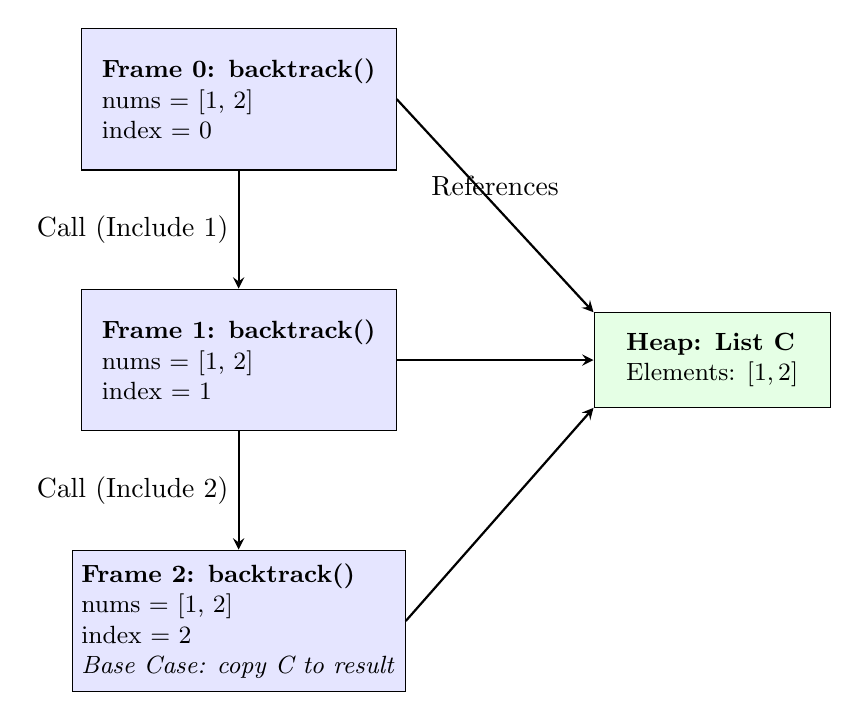
\begin{tikzpicture}[
    node distance=1.5cm and 2.5cm,
    frame/.style={rectangle, draw=black, fill=blue!10, minimum width=4cm, minimum height=1.8cm, align=left, font=\small},
    heap/.style={rectangle, draw=black, fill=green!10, minimum width=3cm, minimum height=1.2cm, align=left, font=\small},
    arrow/.style={-stealth, thick}
]

    % Call stack frames
    \node[frame] (f0) {
        \textbf{Frame 0: backtrack()} \\
        nums = [1, 2] \\
        index = 0
    };
    
    \node[frame] (f1) [below=of f0] {
        \textbf{Frame 1: backtrack()} \\
        nums = [1, 2] \\
        index = 1
    };

    \node[frame] (f2) [below=of f1] {
        \textbf{Frame 2: backtrack()} \\
        nums = [1, 2] \\
        index = 2 \\
        \emph{Base Case: copy C to result}
    };
    
    % Heap variable
    \node[heap] (h) [right=of f1] {
        \textbf{Heap: List C} \\
        Elements: $[1, 2]$
    };

    % Draw connections
    \draw[arrow] (f0) -- (f1) node[midway, left] {Call (Include 1)};
    \draw[arrow] (f1) -- (f2) node[midway, left] {Call (Include 2)};
    \draw[arrow] (f0.east) -- (h.north west) node[midway, above] {References};
    \draw[arrow] (f1.east) -- (h.west);
    \draw[arrow] (f2.east) -- (h.south west);

\end{tikzpicture}
\caption{Visualization of the call stack sharing a single mutable list on the heap.}
\label{fig:stack}
\end{figure}

The call stack forms a chain of activation records. Because Java passes object references by value, the parameter \texttt{current} in all frames points to the exact same \texttt{ArrayList} instance on the heap. 

When \texttt{Frame 2} returns, the CPU pops its activation record. The execution resumes in \texttt{Frame 1} at the instruction immediately following the recursive call:
\begin{verbatim}
current.remove(current.size() - 1); // Backtracking step
\end{verbatim}
If we omit this backtracking step, the list $C$ remains $[1, 2]$. When \texttt{Frame 1} proceeds to its second branch (the "Exclude" decision) and calls \texttt{backtrack(..., index = 2)}, the state is "polluted" because the element $2$ was never removed. The algorithm would generate $[1, 2]$ again, leading to duplicate subsets and incorrect leaf-node outputs. 

Thus, the backtracking step is a strict mathematical and computational requirement to guarantee that the shared state remains in sync with the current path in the state space exploration tree.

\section{Conclusion}
This paper has presented a rigorous examination of the backtracking paradigm, formalizing it as a constrained DFS traversal over combinatorial state trees. We demonstrated how pruning bounds—derived from structural properties like Dyck path constraints—drastically reduce search spaces, converting exponential brute-force searches into highly structured, pruned explorations. Through a low-level systems review, we illustrated that the backtracking step is not merely an algorithmic detail, but an essential mechanism to restore shared memory heap configurations across recursive stack frame transitions.


\end{document}
